%%%%%%%%%%%%%%%%%%%%%%%%%%%%%%%%%%%%%%%%%
%
% PSI Chair Thesis Template
% Version 20200913
%
% based on MastersDoctoralThesis.cls
% Version 2.5 (27/8/17)
%
% which was obtained from:
% http://www.LaTeXTemplates.com
%
% Version 2.x major modifications by:
% Vel (vel@latextemplates.com)
%
% This template is based on a template by:
% Steve Gunn (http://users.ecs.soton.ac.uk/srg/softwaretools/document/templates/)
% Sunil Patel (http://www.sunilpatel.co.uk/thesis-template/)
%
% License of this guide and the template
% CC BY-SA 4.0 (http://creativecommons.org/licenses/by-sa/4.0/)
%
% Exception 1: Some excerpts, figures, and tables that have been taken
% from the literature (denoted with a citation in the caption) are not
% covered by the above license. Permission to re-use and distribute
% these excerpts, figures, and tables must be obtained from the
% respective holder of the copyrights.
%
% Exception 2: Chapter 1 and Appendix C are based on content from the
% MastersDoctoralThesis template mentioned above, which is licensed under
% CC BY-SA 3.0 (http://creativecommons.org/licenses/by-nc-sa/3.0/)
%
% License of the PSIThesis.cls class file:
% LPPL v1.3c (http://www.latex-project.org/lppl)
%
%%%%%%%%%%%%%%%%%%%%%%%%%%%%%%%%%%%%%%%%%

%----------------------------------------------------------------------------------------
%	PACKAGES AND OTHER DOCUMENT CONFIGURATIONS
%----------------------------------------------------------------------------------------
\PassOptionsToPackage{english,ngerman}{babel}
\documentclass[
11pt, % The default document font size is 11 (recommended), options: 10pt, 11pt, 12pt
%oneside, % Two-side layout is recommended; uncomment to switch to one-sided
english, % replace with ngerman for German; not fully supported so far -- requires changes elsewhere
singlespacing, % Single line spacing (recommended), alternatives: onehalfspacing or doublespacing
%draft, % Uncomment to enable draft mode (no pictures, no links, overfull hboxes indicated)
%nolistspacing, % If the document is onehalfspacing or doublespacing, uncomment this to set spacing in lists to single
%liststotoc, % Uncomment to add list of figures/tables/etc to table of contents (not recommended)
%toctotoc, % Uncomment to add the main table of contents to the table of contents (not recommended)
parskip, % add space between paragraphs (recommended)
nohyperref, % do not load the hyperref package (is loaded in setup.tex)
%headsepline, % print a horizontal line under the page header
consistentlayout, % layout of declaration, abstract and acknowledgements pages matches the default layout
%final, % Uncomment to hide all todo notes
]{PSIThesis} % The class file specifying the document structure

% version of the guide
\def\tversion{v20200913}

% long-term stable URL to the thesis guide
\def\doiurl{https://doi.org/10.20378/irb-48428}
\def\githuburl{https://github.com/UBA-PSI/psi-thesis-guide}

%%%%%%%%%%%%%%%%%%%%%%%%%%%%%%%%%%%%%%%%%%%%%%%%%%%
%
% File: setup.tex
%
% This file is part of the PSIThesis.cls
% LaTeX documentclass
%
% The code in this file is made available
% under the following license:
%
% LPPL v1.3c (http://www.latex-project.org/lppl)
%
%%%%%%%%%%%%%%%%%%%%%%%%%%%%%%%%%%%%%%%%%%%%%%%%%%%


%----------------------------------------------------------------------------------------
%		UNIVERSITY OF BAMBERG COLORS
%----------------------------------------------------------------------------------------

% http://www.brandwares.com/RGBTintCalculator.php
% Base Color value obtained from UB Corporate Identity Manual
\definecolor{ubblue}{HTML}{00457D}
\definecolor{ubblue80}{HTML}{336A97}
\definecolor{ubblue60}{HTML}{668FB1}
\definecolor{ubblue40}{HTML}{99B5CB}
\definecolor{ubblue20}{HTML}{CCDAE5}

\definecolor{ubyellow}{HTML}{FFD300}
\definecolor{ubyellow25}{HTML}{FFF4BF}

\definecolor{ubred}{HTML}{e6444F}

\definecolor{ubgreen}{HTML}{97BF0D}

\definecolor{gray75}{gray}{0.75}
\definecolor{gray50}{gray}{0.50}

%----------------------------------------------------------------------------------------
%		FONT SETUP
%----------------------------------------------------------------------------------------

%\usepackage[T1]{fontenc} % Output font encoding for international characters - do not use T1 encoding with luatex!
\usepackage[utf8]{luainputenc} % makes unicode characters like –, €, and ß work properly

% amssymb must be loaded before newtxmath to avoid this error:
% Command `\Bbbk' already defined
\usepackage{amssymb}
\usepackage[cochineal]{newtxmath} % must be loaded before fontspec

\usepackage[no-math]{fontspec} % allows us to use OTF/TTF fonts, but do not interfere with math (because we use newtxmath, which does support Cochineal)

% If you cannot use the cochineal font, uncomment the following lines to select
% the Crimson font. Note, however, that you'll have to take care of the math font
% on your own.
%
%\setmainfont[
%	Path           = fonts/,
%    BoldFont       = {Crimson-Semibold.otf},
%    ItalicFont     = {Crimson-Italic.otf},
%    BoldItalicFont = {Crimson-BoldItalic.otf}
%]{Crimson-Roman.otf}

\setmainfont{Cochineal}[
  Numbers={Proportional,OldStyle},
  Style=Swash % for nice swashed Q letter, see https://golatex.de/spezeielle-opentype-features-in-fontspec-aktivieren-t19831.html
]
%\setmainlanguage{english}
\DeclareSymbolFont{operators}{\encodingdefault}{\familydefault}{m}{n} %  render numbers in cochineal, cf. https://tex.stackexchange.com/questions/398895/using-two-different-math-fonts-with-lualatex

% imitate the behavior of the cochineal package as follows:
% cf. https://tex.stackexchange.com/questions/448895/fontenc-vs-fontspec-with-xelatex
\DeclareRobustCommand{\lfstyle}{\addfontfeatures{Numbers=Lining}}
\DeclareTextFontCommand{\textlf}{\lfstyle}
\DeclareRobustCommand{\tlfstyle}{\addfontfeatures{Numbers={Tabular,Lining}}}
\DeclareTextFontCommand{\texttlf}{\tlfstyle}

% Exception: tables should use "lining figures" (all digits having same width)
\AtBeginEnvironment{tabular}{%
  \tlfstyle
}
\AtBeginEnvironment{tabularx}{%
  \tlfstyle
}


% monospace font, will be used in verbatim and listing environments
\setmonofont[
	Path           = fonts/,
    BoldFont       = {iosevka-ss04-bold.ttf},
    ItalicFont       = {iosevka-ss04-italic.ttf},
    BoldItalicFont       = {iosevka-ss04-bolditalic.ttf},
    Scale = 0.83 % manually determined value;
]{iosevka-ss04-regular.ttf}


% sans-serif font, will be used in the margins
\setsansfont[
	Path          	= fonts/,
	BoldFont		= Roboto-Bold.otf,
	ItalicFont		= Roboto-Italic.otf,
	BoldItalicFont	= Roboto-BoldItalic.otf,
	Scale = 0.83 % manually determined value;
]{Roboto-Regular.otf}

\renewcommand{\familydefault}{\rmdefault}
\defaultfontfeatures{Ligatures=TeX}


%----------------------------------------------------------------------------------------
%		HEADINGS SETUP (CHAPTERS, SECTIONS, …)
%----------------------------------------------------------------------------------------

\usepackage[explicit]{titlesec}
\newcommand{\hsp}{\hspace{20pt}}

\setcounter{secnumdepth}{3}

% We use lining figures for headers (tlfstyle) because they fit better with uppercase letters than old-style figures.

% chapters have a vertical line between number and title
\titleformat{\chapter}[hang]{\Huge\bfseries\tlfstyle}{\color{black}\thechapter}{20pt}{\begin{tabular}[t]{@{\color{ubblue60}\vrule width 2pt\hsp}p{0.85\textwidth}}\raggedright #1\end{tabular}}

% sections
\titleformat{\section}[hang]{\bfseries\large\tlfstyle}{{\color{ubblue}\thechapter.\arabic{section}}}{1ex}{{\color{ubblue} #1}}{}

% subsections
\titleformat{\subsection}[hang]{\bfseries\large\tlfstyle}{{\color{ubblue}\thechapter.\arabic{section}.\arabic{subsection}}}{1ex}{{\color{ubblue} #1}}{}

% subsubsections
\titleformat{\subsubsection}[hang]{\bfseries\tlfstyle}{{\color{ubblue}\thechapter.\arabic{section}.\arabic{subsection}.\arabic{subsubsection}}}{1ex}{{\color{ubblue} #1}}{}

% vertical spacing for headings ==============
\titlespacing*{\section}
{0pt}{7ex}{3ex}

\titlespacing*{\subsection}
{0pt}{4ex}{2ex}

\titlespacing*{\subsubsection}
{0pt}{4ex}{2ex}
% end of vertical spacing ====================

%----------------------------------------------------------------------------------------
%		TABLE OF CONTENTS SETUP
%----------------------------------------------------------------------------------------

% solution inspired from https://tex.stackexchange.com/questions/178510/how-can-i-reproduce-this-beautiful-table-of-contents
\usepackage{etoc}
\etocsetlevel{section}{2}
\etocsetlevel{subsection}{3}

\etocsettocdepth{section} % set to subsection for adding subsections to toc (not recommended)

\newlength{\tocleft}
\setlength{\tocleft}{2.5cm} % must be set to fit the innermargin defined in geometry (change only if you have changed the margins)

\newlength{\tocsep}
\setlength{\tocsep}{2em}

\usepackage{textcase}


\etocsetstyle{chapter}
   {}
   {}
   {\etocifnumbered
     {\makebox[0pt][r]
       % we use \etocthenumber instead of \etocnumber to avoid the href, which is part of \etocthenumber, messing with MakeTextLowercase
       {\textsc{\MakeTextLowercase\chaptername\ \MakeTextLowercase\etocthenumber}\hspace{\tocsep}}%
       \textbf{\etocname\kern1em\relax\etocpage}%
    }%
    {\textbf{\etocname\kern1em\relax\etocpage}}%
    \par\vspace{3ex}%
   }%
   {}

\etocsetstyle{section}
   {\vspace{-2ex}} % Muss von den 3ex aus Chapter abgezogen werden
   {}
   % see the comment regarding etocthenumber in the chapter style definition
   {\makebox[0pt][r]{\textsc{\MakeTextLowercase\etocthenumber}\hspace{\tocsep}}%
    \etocname\kern1em\etocpage\par%
   }%
   {\addvspace{3ex}} % 3ex falls danach Chapter kommt

\etocsetstyle{subsection}
   {\vspace{0ex}}
   {}
   {\makebox[3em][l]{\etocnumber}\etocname\kern1em\etocpage\par}
   {\addvspace{2ex}} % 2ex falls danach Section kommt

\etocsettocstyle{\chapter*{\contentsname}
                \thispagestyle{plain}%
                \leftskip\tocleft\parindent0pt}{}


%----------------------------------------------------------------------------------------
%		OTHER PACKAGES
%----------------------------------------------------------------------------------------

\usepackage{tabularx} % for more flexible tables

\usepackage{marginnote} % Enable Notes on the Page Margin
\usepackage{marginfix} % Enables floating for margin figures
\usepackage{ragged2e} % provides better hyphenation, use with camel case: \RaggedRight
\renewcommand*{\raggedleftmarginnote}{\RaggedLeft}
\renewcommand*{\raggedrightmarginnote}{\RaggedRight}

% justified margin notes:
% uncomment the following two lines to for justified layout of margin notes
%\renewcommand*{\raggedleftmarginnote}{\RaggedLeft}
%\renewcommand*{\raggedrightmarginnote}{\RaggedRight}



\renewcommand*{\marginfont}{\setlength{\parskip}{0.5ex}\scriptsize\sffamily} % format margin text



% for sidenotes: change marginpar font
\usepackage{xparse}
\let\oldmarginpar\marginpar
\RenewDocumentCommand{\marginpar}{om}{%
  \IfNoValueTF{#1}
    {\oldmarginpar{\mymparsetup #2}}
    {\oldmarginpar[\mymparsetup #1]{\mymparsetup #2}}}
\newcommand{\mymparsetup}{\scriptsize\sffamily}


% this provides correct alignment for margin text that is inserted
% right at the beginning of a paragraph; however, it messes up the
% alignment in all other cases.
%% therefore, removed for now:
%%\renewcommand{\marginnotevadjust}{0.71\baselineskip}
% The following is the necessary correction for in-paragraph use
\renewcommand{\marginnotevadjust}{0.21\baselineskip}
\renewcommand{\marginnotevadjust}{0.55\baselineskip}

\usepackage{microtype} % enable better typographic setup

\usepackage{multicol} % enable usage of multiple columns

% biblatex setup
% inspired by https://anneurai.net/2017/10/18/thesis-formatting-in-latex/
\usepackage[
  backend=biber,
  style=alphabetic,
  doi=false,isbn=false, % these fields are commonly omitted
  terseinits=true, % no points between initials
  giveninits=true, % always print only initials for given names
  sortcites=true,
  language=english,
  backref=true, % show on what pages a ref has been cited
  maxcitenames=2, % how many names the \citeauthor will show
]{biblatex} % Use biber backend with alphabetic reference style
\AtEveryBibitem{%
  \clearlist{language} % don't show "en."
  \clearlist{extra} % clears extra fields such as ISBN nrs
}

% shorten the strings used in back references
\DefineBibliographyStrings{english}{%
  backrefpage = {page},
  backrefpages = {pages},
}

%-- no "quotes" around titles of chapters/article titles
\DeclareFieldFormat[article, inbook, incollection, inproceedings, misc, thesis, unpublished]{title}{#1}
%-- no punctuation after volume
\DeclareFieldFormat[article]{volume}{{#1}}
%-- puts number/issue between brackets
\DeclareFieldFormat[article, inbook, incollection, inproceedings, misc, thesis, unpublished]{number}{\mkbibparens{#1}}
%-- and then for articles directly the pages w/o any "pages" or "pp."
\DeclareFieldFormat[article]{pages}{#1}
%-- format 16(4):224--225 for articles
\renewbibmacro*{volume+number+eid}{\printfield{volume}\printfield{number}\printunit{\addcolon}
}
\DeclareFieldFormat{url}{\url{#1}}


\usepackage[autostyle=true]{csquotes} % Required to generate language-dependent quotes in the bibliography

\usepackage[
  obeyFinal,
  textsize=scriptsize,
  backgroundcolor=ubyellow25,linecolor=ubyellow,bordercolor=ubyellow,
]{todonotes}

% change font of todo notes to sans-serif
\makeatletter
\renewcommand{\todo}[2][]{\@bsphack\@todo[#1]{\sffamily #2}\@esphack\ignorespaces}
\makeatother

\usepackage{booktabs} % use formal table layout

\urlstyle{same} % avoids printing URLs in typewriter font

% enable very extensive URL breaking
% https://tex.stackexchange.com/questions/3033/forcing-linebreaks-in-url
\PassOptionsToPackage{hyphens}{url}
\expandafter\def\expandafter\UrlBreaks\expandafter{\UrlBreaks% save the current one
  \do\a\do\b\do\c\do\d\do\e\do\f\do\g\do\h\do\i\do\j%
  \do\k\do\l\do\m\do\n\do\o\do\p\do\q\do\r\do\s\do\t%
  \do\u\do\v\do\w\do\x\do\y\do\z\do\A\do\B\do\C\do\D%
  \do\E\do\F\do\G\do\H\do\I\do\J\do\K\do\L\do\M\do\N%
  \do\O\do\P\do\Q\do\R\do\S\do\T\do\U\do\V\do\W\do\X%
  \do\Y\do\Z\do\*\do\-\do\~\do\'\do\"\do\-}%

% TODO consider using package xurl, which is supposed to handle url breaking

% https://tex.stackexchange.com/a/450695
% allow URLs to be spaced out at / => much better URL breaking in margins
\makeatletter
\g@addto@macro\UrlSpecials
{%
    \do\/{\mbox{\UrlFont/}\hskip 0pt plus 0.1em minus 0.1em}%
}
\Urlmuskip=0mu plus 1mu\relax
\makeatother


% hyperlink layout
\usepackage{hyperref}
 \hypersetup{colorlinks,breaklinks,unicode,
             citecolor=ubblue60,
             linkcolor=ubblue60,
             filecolor=ubblue60,
             urlcolor=ubblue60}

% cleverref allows you to use \Cref{sec:foo} to get the text "Section 1.2".
% This also works with figures and tables.
\usepackage{cleveref}

% datetime is use to automatically handle the date rendering on the titlepage.
\usepackage{datetime}
% rendering the current date as Month/JJJJ
% see: https://tex.stackexchange.com/questions/212263/month-year-format-in-latex
\newdateformat{monthyeardate}{%
  \monthname[\THEMONTH] \THEYEAR}


\raggedbottom % do NOT force all pages to have the same height (which would be done by increasing the space between paragraphs, which can create noisy layouts)

%----------------------------------------------------------------------------------------
%	SETUP BIBLIOGRAPHY
%----------------------------------------------------------------------------------------
\setlength{\bibitemsep}{.3\baselineskip plus .05\baselineskip minus .05\baselineskip}
\newlength{\bibparskip}\setlength{\bibparskip}{0pt}
\let\oldthebibliography\thebibliography
\renewcommand\thebibliography[1]{%
  \oldthebibliography{#1}%
  \setlength{\parskip}{\bibitemsep}%
  \setlength{\itemsep}{\bibparskip}%
}

% allow much more liberal line breaks in URLs
\setcounter{biburllcpenalty}{7000}
\setcounter{biburlucpenalty}{8000}

% adjust space between key and entry, default is 2\labelsep
\setlength{\biblabelsep}{1\labelsep}

% configures indentation of bibentries
\defbibenvironment{bibliography}
  {\list
     {\hspace{0.5\labelalphawidth}\bfseries\printtext[labelalphawidth]{%
        \printfield{prefixnumber}%
        \printfield{labelalpha}%
        \printfield{extraalpha}}}
     {\setlength{\labelsep}{\biblabelsep}%
      \setlength{\leftmargin}{0.5\labelalphawidth}%
      \setlength{\itemsep}{1.5\bibitemsep}%
      \setlength{\parsep}{\bibparsep}}%
      \renewcommand*{\makelabel}[1]{##1\hss}}
  {\endlist}
  {\item}


%----------------------------------------------------------------------------------------
%	MARGIN SETTINGS
%----------------------------------------------------------------------------------------

% Using the layout from kaobook
\geometry{
		paper=a4paper,
		head=13.6pt,
		top=27.4mm,
		bottom=27.4mm,
		inner=24.8mm,
		%outer=24.8mm,
		%right=2.183cm,
		textwidth=107mm,
		marginparsep=8.2mm,
		marginparwidth=49.4mm,
		%textheight=49\baselineskip,
		includemp,
		% showframe
}

% Wide figures span text and margin.
% Use the pre-calculated length \widefigurewidth in \includegraphics.
\def\widefigurewidth{\dimexpr(\marginparwidth + \textwidth + \marginparsep)}


%----------------------------------------------------------------------------------------
%	SETUP HEADER AND FOOTER
%----------------------------------------------------------------------------------------


\newlength{\overflowingheadlen}
\setlength{\overflowingheadlen}{\textwidth}
\addtolength{\overflowingheadlen}{\marginparsep}
\addtolength{\overflowingheadlen}{\marginparwidth}

% old header/footer, maybe not necessary any more?
% \automark[chapter]{chapter}
% \ihead{\textup{\headmark}} % Inner header; do not use italics: therefore textup
% \ihead{\textup{\textsc{\MakeLowercase\headmark}}}% Inner header - use this line for Small Caps in header
% \ohead[]{\pagemark} % Outer header
% \cfoot[\pagemark]{} % On chapter opening pages, the page number goes centered into the footer
% \automark*[section]{}%

% new header/footer, from kaobook; we could probably remove the original definitions from the cls
\renewpagestyle{thesis}{
  {\hspace{-\marginparwidth}\hspace{-\marginparsep}\makebox[\overflowingheadlen][l]{\textup{\thepage}\quad\rule[-\dp\strutbox]{1pt}{\baselineskip}\quad{}\textup{\textsc{\MakeLowercase \leftmark}}}} % left page two sided
  {\makebox[\overflowingheadlen][r]{\textup{\textsc{\MakeLowercase \rightmark}}\quad\rule[-\dp\strutbox]{1pt}{\baselineskip}\quad\textup{\thepage}}} % right page two sided
  % TODO ifthispageodd appears to not effect the header of even/odd pages in onesided layouts
  {\ifthispageodd{\makebox[\overflowingheadlen][l]{\textup{\thepage}\quad\rule[-\dp\strutbox]{1pt}{\baselineskip}\quad{}\textup{\textsc{\MakeLowercase \leftmark}}}}{\makebox[\overflowingheadlen][l]{\textup{\thepage}\quad\rule[-\dp\strutbox]{1pt}{\baselineskip}\quad{}\textup{\textsc{\MakeLowercase \rightmark}}}}} % one sided       
}{
  {}%
  {}%
  {}
}
\renewpagestyle{plain.thesis}{
  {}%
  {}%
  {}
}{
  {\hspace{-\marginparwidth}\hspace{-\marginparsep}\makebox[\overflowingheadlen][l]{\textup{\textsc{\thepage}}\quad\rule[-\dp\strutbox]{1pt}{\baselineskip}}} % left page two sided
  {\makebox[\overflowingheadlen][r]{\rule[-\dp\strutbox]{1pt}{\baselineskip}\quad\textup{\textsc{\thepage}}}} % right page two sided
  {\makebox[\overflowingheadlen][l]{\textup{\textsc{\thepage}}\quad\rule[-\dp\strutbox]{1pt}{\baselineskip}}} % one sided
}

%----------------------------------------------------------------------------------------
%	LISTINGS SETTINGS
%----------------------------------------------------------------------------------------

\usepackage{textcomp}
\usepackage{listings}
\definecolor{darkgray}{rgb}{.4,.4,.4}

\lstdefinelanguage{JavaScript}{
  keywords={typeof, new, true, false, catch, function, return, null, catch, switch, var, if, in, while, do, else, case, break},
  ndkeywords={class, export, boolean, throw, implements, import, this},
  sensitive=false,
  comment=[l]{//},
  morecomment=[s]{/*}{*/},
  morestring=[b]',
  morestring=[b]"
}

\lstset{
    aboveskip={1\baselineskip},
    abovecaptionskip=-1\baselineskip,
    belowcaptionskip=2ex,
    basicstyle=\footnotesize\ttfamily\linespread{4},
    breaklines=true,
    columns=flexible,
    commentstyle=\color{gray50}\ttfamily\itshape,
    escapechar=@,
    extendedchars=true,
    frame=l,
    framerule=.5pt,
    identifierstyle=\color{black},
    inputencoding=latin1,
    keywordstyle=\color{ubblue80}\bfseries,
    ndkeywordstyle=\color{ubblue80}\bfseries,
    numbers=left,
    numbersep=1.25em,
    numberstyle=\scriptsize\ttfamily,
    prebreak = \raisebox{0ex}[0ex][0ex]{\ensuremath{\hookleftarrow}},
    stringstyle=\color{ubblue60}\ttfamily,
    upquote=true,
    showstringspaces=false,
}

\lstset{literate=%
   *{0}{{{\color{darkgray}0}}}1
    {1}{{{\color{darkgray}1}}}1
    {2}{{{\color{darkgray}2}}}1
    {3}{{{\color{darkgray}3}}}1
    {4}{{{\color{darkgray}4}}}1
    {5}{{{\color{darkgray}5}}}1
    {6}{{{\color{darkgray}6}}}1
    {7}{{{\color{darkgray}7}}}1
    {8}{{{\color{darkgray}8}}}1
    {9}{{{\color{darkgray}9}}}1
}

\lstnewenvironment{latex}
    {\lstset{language=[LaTeX]TeX}}
    {}

%----------------------------------------------------------------------------------------
%	MARGINAL CAPTIONS
%----------------------------------------------------------------------------------------

\usepackage{sidenotes}
\usepackage{scrextend} % for ifthispageodd

% objective: instead of having the sidenode number in superscript, we want it like "1:"
\makeatletter
\ExplSyntaxOn
\RenewDocumentCommand \sidenotetext { o o +m }
{
  \IfNoValueOrEmptyTF{#1}
    {
      \@sidenotes@placemarginal{#2}{\thesidenote{}:~#3}
  \refstepcounter{sidenote}
}
    {\@sidenotes@placemarginal{#2}{#1{}:~#3}}
}
\ExplSyntaxOff
\makeatother

% optional objective: automatically justify sidecaptions to match the other marginnotes
% captions of marginfigures etc. shall always be raggedright
% solution from: https://tex.stackexchange.com/questions/358010/subfigures-break-figure-numbering-with-sidecaptions-from-sidenotes-package/358012#358012

\makeatletter
% Instead of "justified" you *can* use "outerraged" in the DeclareCaptionStyle below.
% This may create a inconsistent layout, therefore, we stick to justified by default.
\DeclareCaptionJustification{outerragged}{\ifthispageodd{\RaggedRight}{\RaggedLeft}}

\DeclareCaptionStyle{sidecaption}{format=plain,font={scriptsize,sf},labelfont=bf,margin=0pt,singlelinecheck=true,justification=justified}
\DeclareCaptionStyle{marginfigure}{format=plain,font={scriptsize,sf},labelfont=bf,margin=0pt,singlelinecheck=true}
\DeclareCaptionStyle{margintable}{format=plain,font={scriptsize,sf},labelfont=bf,margin=0pt,singlelinecheck=true}
\DeclareCaptionStyle{widefigure}[justification=centering]{format=plain,font=small,labelfont=bf,justification=RaggedRight,singlelinecheck=true,margin={0px,0px},oneside}
\DeclareCaptionStyle{widetable}[justification=centering]{format=plain,font=small,labelfont=bf,justification=RaggedRight,singlelinecheck=true,margin={0px,0px},oneside}
\makeatother


%----------------------------------------------------------------------------------------
%	RESET SIDENOTE COUNTER AT EVERY CHAPTER
%----------------------------------------------------------------------------------------

\let\oldchapter\chapter
\def\chapter{%
  \setcounter{sidenote}{1}%
  \oldchapter
}


%----------------------------------------------------------------------------------------
%	SYMBOLS
%----------------------------------------------------------------------------------------

\usepackage{pifont}
\let\oldding\ding% Store old \ding in \oldding
\renewcommand{\ding}[2][1]{\scalebox{#1}{\oldding{#2}}}% Scale \oldding via optional argument
% usage \ding{number} or |ding[factor]{number}


%----------------------------------------------------------------------------------------
%	ITEMIZE AND ENUMERATE ENVIRONMENTS
%----------------------------------------------------------------------------------------

\renewcommand{\labelitemi}{\color{ubblue80}{\scalebox{0.8}{\raisebox{0.2ex}{$\blacktriangleright$}}}}
\renewcommand{\labelitemii}{\textbullet}
\usepackage{enumitem}
\setlist[itemize]{parsep=0.8\parskip,left=0pt,topsep=0pt,partopsep=0pt}
\setlist[enumerate]{parsep=0.8\parskip,left=0pt,topsep=0pt,partopsep=0pt}
\setlist[description]{parsep=0.8\parskip,left=0pt,topsep=0pt,partopsep=0pt}


%----------------------------------------------------------------------------------------
%	SET PDF METADATA
%----------------------------------------------------------------------------------------

\AtBeginDocument{
\hypersetup{pdftitle=\ttitle} % Set the PDF's title to your title
\hypersetup{pdfauthor=\authorname} % Set the PDF's author to your name
%\hypersetup{pdfkeywords=\keywordnames} % Set the PDF's keywords to your keywords
}
 % Load the settings from Misc/setup.tex
%%%%%%%%%%%%%%%%%%%%%%%%%%%%%%%%%%%%%%%%%%%%%%%%%%%
%
% File: commands.tex
% 
% This file is part of the PSIThesis.cls
% LaTeX documentclass
% 
% The code in this file is made available
% under the following license:
%
% LPPL v1.3c (http://www.latex-project.org/lppl)
%
%%%%%%%%%%%%%%%%%%%%%%%%%%%%%%%%%%%%%%%%%%%%%%%%%%%


% --------------------------------------------------------
% 			CUSTOM COMMANDS FOR BETTER USABILITY
% --------------------------------------------------------


% Custom image command to insert an image
% This command uses 4 required and one optional arguments/parameters with the following meaning:
%
% Optional:
% 1 - Position of the figure (the default position is 't' for top; if no argument is provided, 't' is used
%
% Required:
% 1 - Width of the image
% 2 - Path to the image (inside the figures folder)
% 3 - Caption of the image
% 4 - Label for the image (a universal fig: is prepended)
%
% Required ----------------------------------------------------------------------------
% Optional -------------|		|			  |					|					  |
% 						V		V (1)		  V	(2)				V (3)				  V (4)
% Example Usage: \image[h]{\textwidth}{barplot-before}{This is a fancy barplot.}{barplot-before}
%
% The result will be the same as:
%
% \begin{figure}[h]
% 	\centering
% 	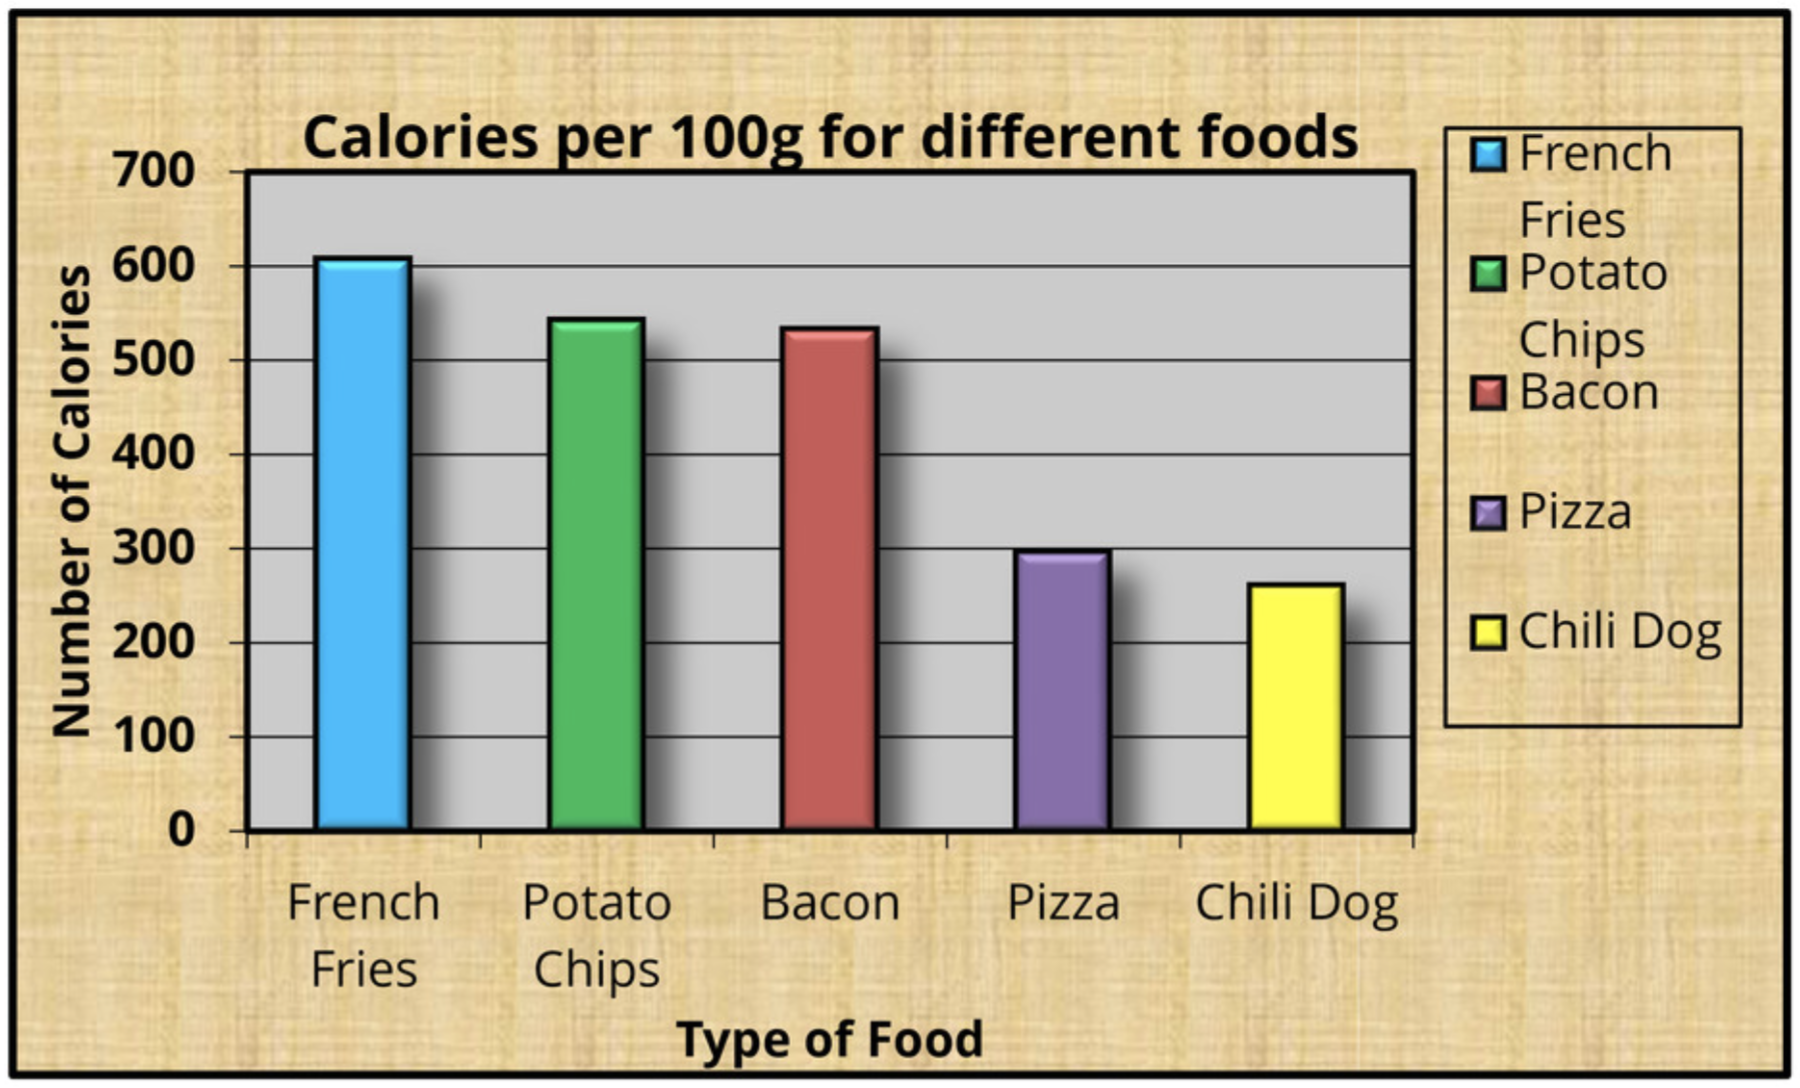
\includegraphics[width=\textwidth]{../figures/barplot-before}
% 	\caption{This is a fancy barplot.}
% 	\label{fig:barplot-before}
% \end{figure}

\newcommand{\image}[5][t]{
	\begin{figure}[#1]
		\centering
		\includegraphics[width=#2]{../figures/#3}
		\caption{#4}
		\label{fig:#5}
	\end{figure}
}

% Custom command to insert two images next to each other with a margin caption
% This command uses 6 required and one optional arguments/parameters with the following meaning:
%
% Optional:
% 1 - Position of the figure (the default position is 't' for top; if no argument is provided, 't' is used
%
% Required:
% 1 - Path to the frist image (inside the figures folder)
% 2 - Path to the second image (inside the figures folder)
% 3 - Caption of the image
% 4 - Label for the image (a universal fig: is prepended)
%
% Required --------------------------------------------------------------------------------------
% Optional -----------------|		  |			    |					|					    |
% 						    V		  V (1)		    V (2)				V (3)				    V (4)
% Example Usage: \twoimages[h]{barplot-before}{barplot-after}{This is a fancy barplot.}{barplot-sidebyside}
%
% The result will be the same as:
%
% \begin{figure}[h]
% 	\centering
% 	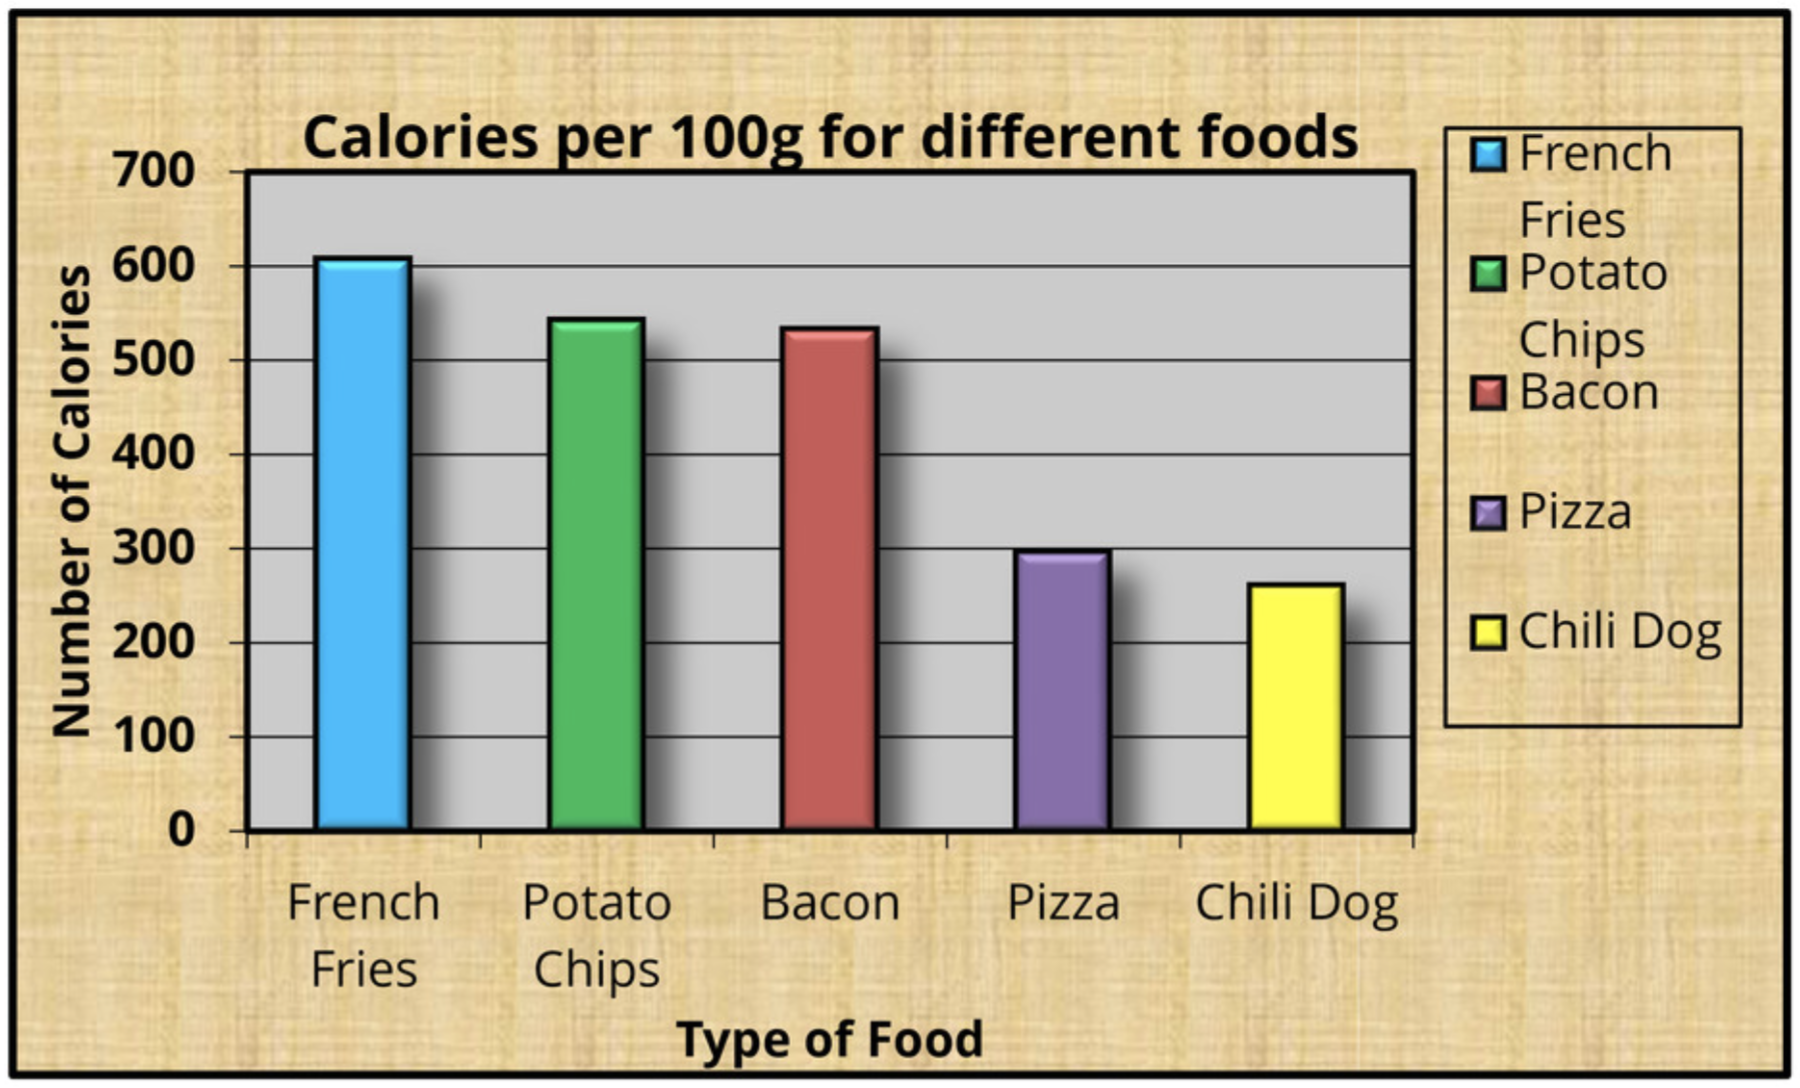
\includegraphics[width=0.48\textwidth]{../figures/barplot-before}
% 	\hspace{\fill}
% 	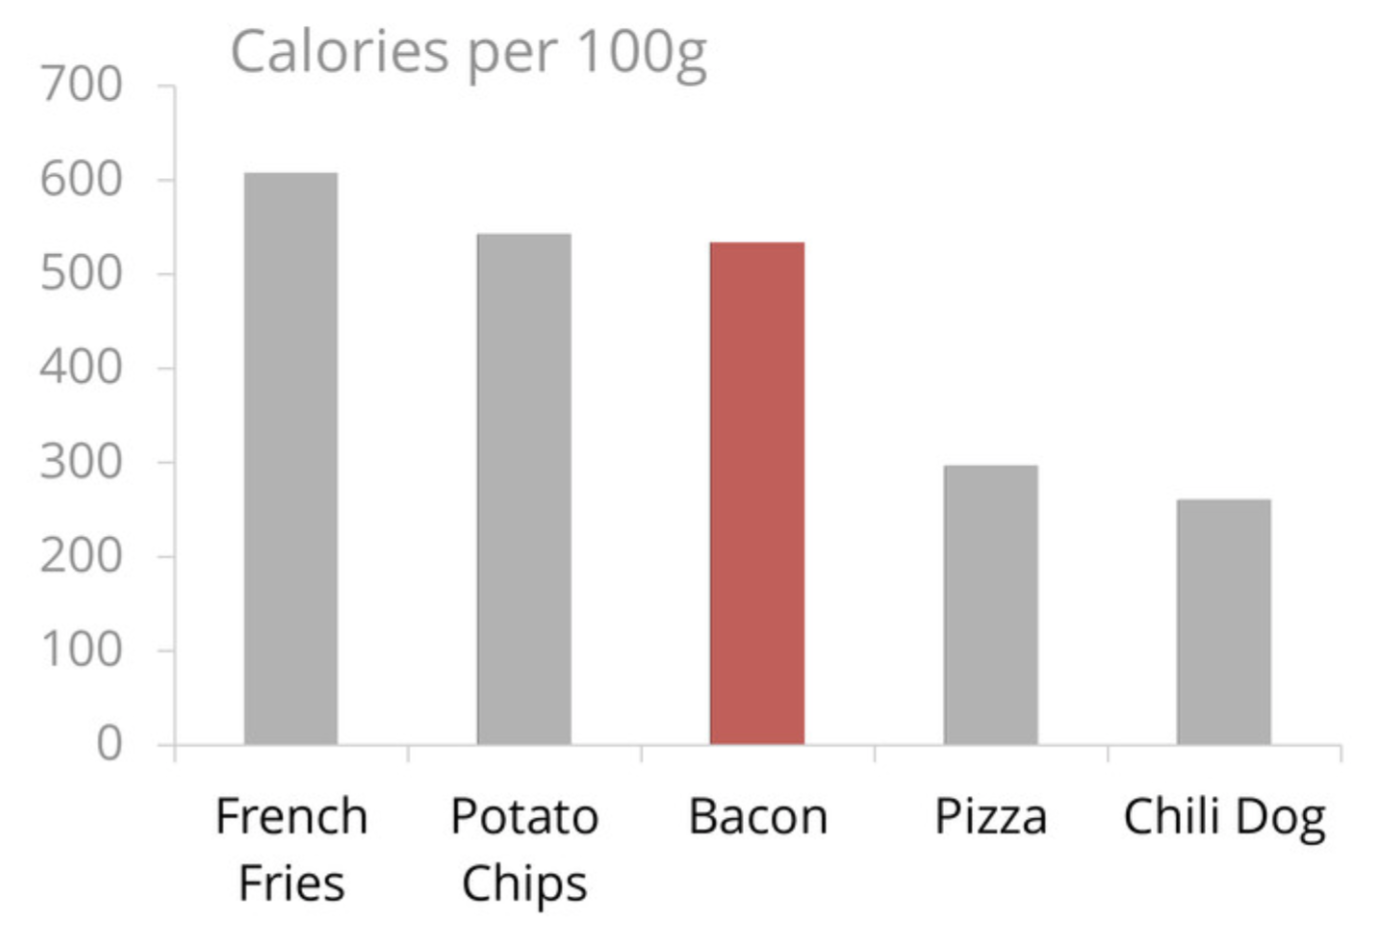
\includegraphics[width=0.48\textwidth]{../figures/barplot-after}
% 	\caption{\label{fig:barplot-sidebyside}This is a fancy barplot.}
% \end{figure}

\newcommand{\twoimages}[5][t]{
	\begin{figure}[#1]
		\centering
		\includegraphics[width=0.48\textwidth]{../figures/#2}
		\hspace{\fill}
		\includegraphics[width=0.48\textwidth]{../figures/#3}
		\sidecaption{\label{fig:#5}#4}[-2\baselineskip]
	\end{figure}
}


% Custom image command for wide figures
% This command uses 4 required and one optional arguments/parameters with the following meaning:
%
% Optional:
% 1 - Position of the figure (the default position is 't' for top; if no argument is provided, 't' is used
%
% Required:
% 1 - Path to the image (inside the figures folder)
% 2 - Caption of the image
% 3 - Label for the image (a universal fig: is prepended)
%
% Required ------------------------------------------------------------------
% Optional -----------------|		  |				 	 |					|
% 						    V		  V (1)		 	  	 V	(2)				V (3)
% Example Usage: \wideimage[h]{barplot-before}{This is a fancy barplot.}{barplot-before}
%
% The result will be the same as:
%
% \begin{figure*}[h]
% 	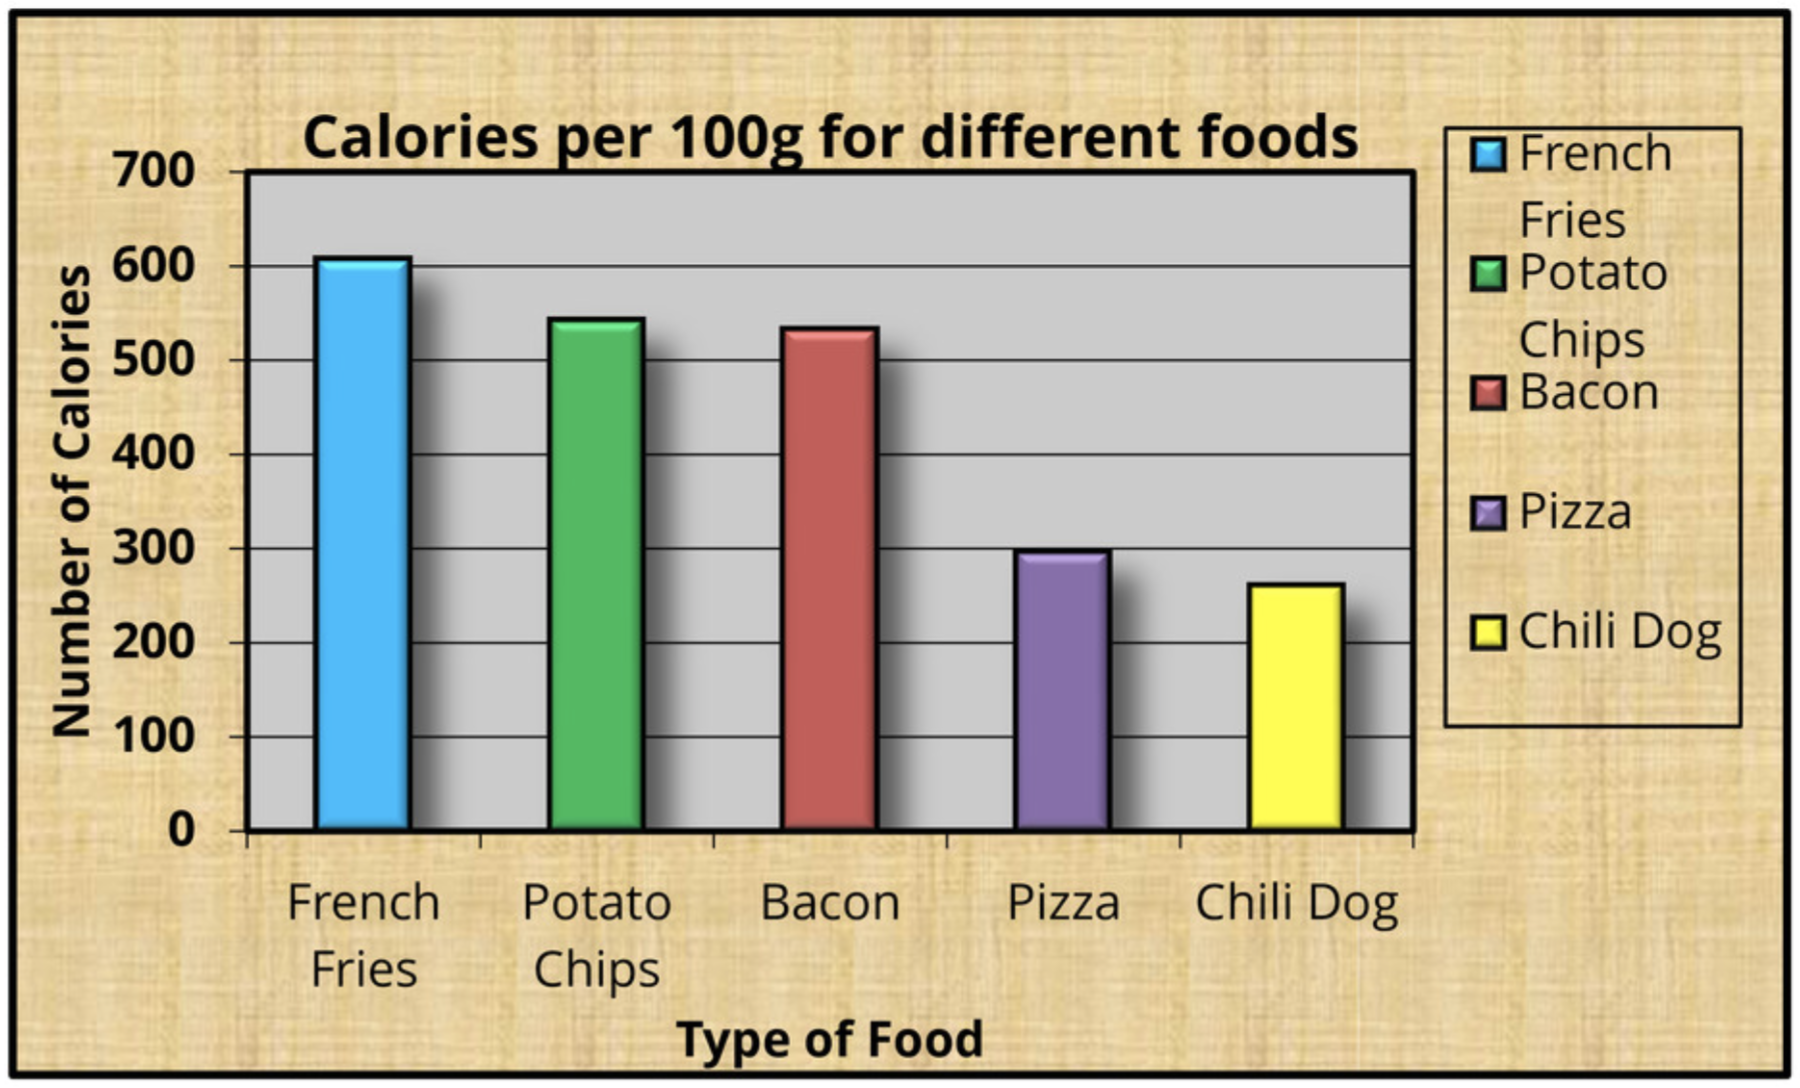
\includegraphics[width=\widefigurewidth]{../figures/barplot-before}
% 	\caption{This is a fancy barplot.}
% 	\label{fig:barplot-before}
% \end{figure*}
%
% %%%%%%%%%%%%%%%%%%%%%%%
% % 	ATTENTION		%
% %%%%%%%%%%%%%%%%%%%%%%%
% It seems this command messes with the position of other images, therefore it is advised to check the placement of other images.

\newcommand{\wideimage}[4][t]{
	\begin{figure*}[#1]
		\includegraphics[width=\widefigurewidth]{../figures/#2}
		\caption{\label{fig:#4}#3}
	\end{figure*}
}

% This command uses 3 required and one optional arguments/parameters with the following meaning:
%
% Optional:
% 1 - Vertical offset of the figure (the default offset is 1 for one line lower (negative numbers move the image up); if no argument is provided, 1 is used
%
% Required:
% 1 - Path to the image (inside the figures folder)
% 2 - Caption of the image
% 3 - Label for the image (a universal fig: is prepended)
%
% Required ----------------------------------------------------------------------
% Optional -------------------|			|				  |						|
% 							  V			V (1)			  V	(2)					V (3)
% Example Usage: \marginimage[2]{barplot-before}{This is a fancy barplot.}{barplot-before}
%
% The result will be the same as:
%
% \begin{marginfigure}[2\baselineskip]
% 	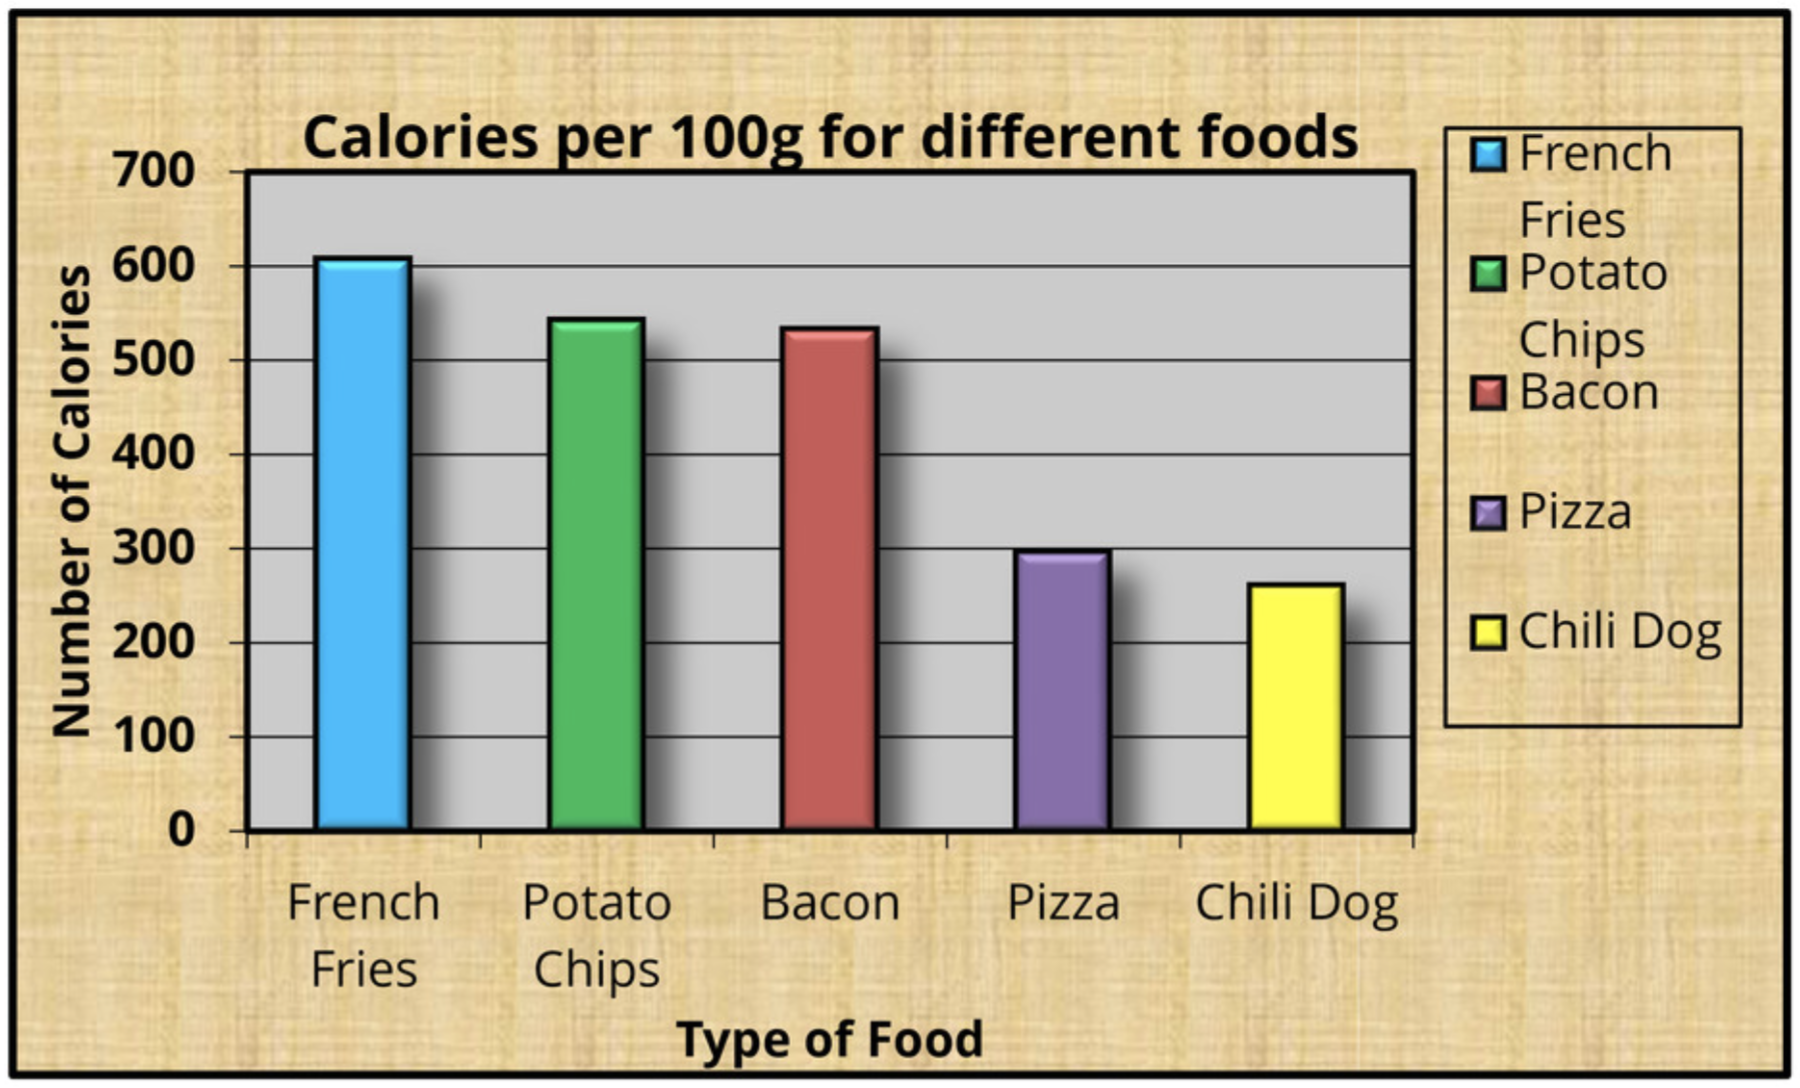
\includegraphics[width=\marginparwidth]{../figures/barplot-before}
% 	\caption{\label{fig:barplot-before}This is a fancy barplot.}
% \end{marginfigure}
\newcommand{\marginimage}[4][1]{
	\begin{marginfigure}[#1\baselineskip]
		\includegraphics[width=\marginparwidth]{../figures/#2}
		\caption{\label{fig:#4}#3}
	\end{marginfigure}
}
 % Load the custom commands from Misc/commands.tex

% Uncomment this command to make all links black:
%   useful for printing on black-white printers that do a
%   poor job at rasterizing colored text properly
%\hypersetup{colorlinks=false}

\addbibresource{literature.bib} % The filename of the bibliography

\usepackage{bytefield}
\usepackage{calc}

%----------------------------------------------------------------------------------------
%	THESIS INFORMATION
%----------------------------------------------------------------------------------------
\newcommand{\thesistype}{Bachelor} % type of your thesis (Bachelors, Masters, Doctoral ...)

%%% CHANGE THIS:
% Your thesis title, this is used in the title and abstract, print it elsewhere with \ttitle
\thesistitle{Alternatives for Virtual Memory Management}

% date to be printed on the title, this will automatically update and be in the correct format
% If any changes to this format (Month JJJJ) are necessary the definition can be found in line 337
% of misc/setup.tex
\def\tdate{\monthyeardate\today}

%%% CHANGE THIS:
% Your name, this is used in the title page, print it elsewhere with \authorname
\author{Max Meidinger}

% Your supervisor's name, this is used in the title page, print it elsewhere with \supname
\supervisor{Prof. Dr. XXX YYY}

% Your university's name and URL, this is used in the title page, print it elsewhere with \univname
\university{\href{https://www.uni-bamberg.de/en/}{University of Bamberg}}

% Your research group's name and URL, this is used in the title page, print it elsewhere with \groupname
\group{\href{https://www.uni-bamberg.de/en/psi/}{Privacy and Security in Information Systems Group}}

% Your department's name and URL, this is used in the title page, print it elsewhere with \deptname
\department{department not used}

% Your faculty's name and URL, this is used in the title page, print it elsewhere with \facname
% TODO: insert *your* degree program in the \faculty command below
% Applied Computer Science
% Computing in the Humanities
% Information Systems
% International Information Systems Management
% International Software Systems Science
% Software Systems Science
% Education in Business and Information Systems
\faculty{Software Systems Science Degree Program in the\\ \href{https://www.uni-bamberg.de/en/wiai/}{Faculty of Information Systems and Applied Computer Sciences}}

% Your address, this is not currently used anywhere in the template, print it elsewhere with \addressname
\addresses{address not used}

% Your subject area, this is not currently used anywhere in the template, print it elsewhere with \subjectname
\subject{subject not used}

% Keywords for your thesis, this is not currently used anywhere in the template, print it elsewhere with \keywordnames
\keywords{keywords not used}
%----------------------------------------------------------------------------------------
%	END OF THESIS INFORMATION
%----------------------------------------------------------------------------------------


\begin{document}

\selectlanguage{english}

\frenchspacing % do not add additional hspace after end of sentence full stop dot.

\frontmatter % Uses roman page numbering style (i, ii, iii, iv...) for the pre-content pages

\hypersetup{urlcolor=black}

%%%%%%%%%%%%%%%%%%%%%%%%%%%%%%%%%%%%%%%%%%%%%%%%%%%
%
% File: titlepage.tex
%
% This file is part of the PSIThesis.cls
% LaTeX documentclass
%
% The code in this file is made available
% under the following license:
%
% LPPL v1.3c (http://www.latex-project.org/lppl)
%
%%%%%%%%%%%%%%%%%%%%%%%%%%%%%%%%%%%%%%%%%%%%%%%%%%%


\pagestyle{plain} % Default to the plain heading style until the thesis style is called for the body content

%----------------------------------------------------------------------------------------
%	TITLE PAGE
%----------------------------------------------------------------------------------------

\begin{titlepage}

	\newgeometry{
		inner=4cm, % Inner margin
		outer=4cm, % Outer margin
		marginparwidth=0cm,
		marginparsep=0mm,
		bindingoffset=.5cm, % Binding offset
		top=2.5cm, % Top margin
		bottom=2.5cm, % Bottom margin
		showframe % Uncomment to show how the type block is set on the page
	}

	\begin{center}

		\vspace*{.06\textheight}

		% The logo of University of Bamberg. Do not use the logo without permission.
		% Using it on the title page of a thesis is acceptable.
		% TODO Add your own logo here. Do yourself and your readers a favor and use
		%      a vectorized logo (PDF) instead of a bitmap (PNG, JPEG)
		
\includegraphics[width=35mm]{misc/UB_Logo_20mm_CMYK.pdf}

		\vspace*{.06\textheight}

		{\LARGE \textls[130]{\MakeUppercase{\univname}}\par}\vspace{2\baselineskip} % University name

		% TODO uncomment the next line when you write a thesis to display the supervisor
		%{\large \facname}
		% TODO comment out the next line when you write a thesis
		{\large ~} % For use in the guide

		\vspace{1.5cm}

		% TODO uncomment the next line when you write a thesis to display the supervisor
		%\textsc{\Large \thesistype 's~Thesis}\\[1cm] % For use in the thesis
		% TODO comment out the next line when you write a thesis
		\textsc{\Large ~}\\[1cm] % For use in the guide

		%\HRule \\[0.4cm] % Horizontal line
		%
		{\huge \bfseries \ttitle\par}\vspace{1cm} % Thesis title

		%\HRule \\[1.5cm] % Horizontal line


		\textsc{\Large by}\\[1cm]

		{\Large \authorname}

		\vspace{1.5cm}

		% TODO uncomment the next two lines when you write a thesis to display the supervisor
		\emph{Supervisor:} \\
		\supname\\[1cm]
		%%

		\groupname%\\[2cm] % Research group name and department name

		\vfill

		{\large \tdate} % Date

		% TODO remove the following lines when you write a thesis
		% \vspace{0.25ex}

		% {\small \tversion}

		% \vspace{0.25ex}

		% {\small Links to this document:}\\
		% {\small \url{\doiurl}} (initial version)\\
		% {\small \url{\githuburl} (most recent version)}
		% Remove lines up to this line

		\vfill
	\end{center}

	\restoregeometry

\end{titlepage}


 % Typeset the titlepage

\hypersetup{urlcolor=ubblue80}


%----------------------------------------------------------------------------------------
%	QUOTATION
%----------------------------------------------------------------------------------------

% \vspace*{0.2\textheight}

% \noindent\enquote{\itshape Thanks to my solid academic training, today I can write hundreds of words on virtually any topic without possessing a shred of information, which is how I got a good job in journalism.}\bigbreak

% \hfill Dave Barry


%----------------------------------------------------------------------------------------
%	ABSTRACT PAGE
%----------------------------------------------------------------------------------------

\begin{abstract}
	%\addchaptertocentry{\abstractname}
	% uncomment to add the abstract to the table of contents (not recommended)

	For an overview of this document, see \Cref{Chapter1}.

	Provide a Thesis Abstract here (length: less than one page).

	For a start, you may want to consult the concise instructions for writing the Summary Paragraph in \emph{Nature}: \url{https://www.nature.com/documents/nature-summary-paragraph.pdf}. Moreover, consider Markus Kuhn's advice on differentiating abstract and introduction: \url{https://www.lightbluetouchpaper.org/2007/03/14/how-not-to-write-an-abstract/}.

	A boilerplate scheme for an abstract is as follows: devote 25\,\% of the space on the purpose and importance of the research (introduction), 25\,\% of the space on what you did (methods), 35\,\% of the space on what you found (results), and 15\,\% of the space on the implications of the research (cf. \url{https://writingcenter.gmu.edu/guides/writing-an-abstract}).

	More concrete advice for writing abstracts can be found on the website of the Writing Center of the University of North Carolina at Chapel Hill (\url{https://writingcenter.unc.edu/tips-and-tools/abstracts/}). Some useful phrases for abstracts can be found at \url{http://dissertation.laerd.com/useful-phrases-when-writing-a-dissertation-abstract.php}

	Finally, you may also want to consider the excellent guide by Kent Beck on how to write good abstracts, which focuses on conference papers:
	\url{https://plg.uwaterloo.ca/~migod/research/beckOOPSLA.html}.

\end{abstract}


%----------------------------------------------------------------------------------------
%	ACKNOWLEDGEMENTS
%----------------------------------------------------------------------------------------

%\begin{acknowledgements}
% %\addchaptertocentry{\acknowledgementname}
% Add the acknowledgements to the table of contents (not recommended)
%
%The acknowledgments and the people to thank go here.
%\end{acknowledgements}


%----------------------------------------------------------------------------------------
%	TABLE OF CONTENTS
%----------------------------------------------------------------------------------------

\cleardoublepage

% Table of Contents uses a wider layout than the main content
\newgeometry{
	head=13.6pt,
	top=27.4mm,
	bottom=27.4mm,
	inner=24.8mm,
	outer=24.8mm,
	marginparsep=0mm,
	marginparwidth=0mm,
}
{
	\hypersetup{linkcolor=black}
	\tableofcontents % Prints the ToC entries
}
\restoregeometry

%----------------------------------------------------------------------------------------
%	DEDICATION
%----------------------------------------------------------------------------------------

% \dedicatory{For/Dedicated to/To my\ldots}


%----------------------------------------------------------------------------------------
%	THESIS CONTENT - CHAPTERS
%----------------------------------------------------------------------------------------
\mainmatter % From here on, numeric (1,2,3...) page numbering
\pagestyle{thesis} % Return the page headers back to the "thesis" style

% Define some commands to keep the formatting separated from the content
\newcommand{\keyword}[1]{\textbf{#1}}
\newcommand{\tabhead}[1]{\textbf{#1}}
\newcommand{\code}[1]{\texttt{#1}}
\newcommand{\file}[1]{\texttt{#1}}
\newcommand{\option}[1]{\texttt{\itshape#1}}

% Figures will automatically be searched for in the Figures subdirectory
\graphicspath{{./figures/}{./examples/}}

%%% CHANGES NEEDED HERE
%
% Include the chapters of the thesis as separate files from the Chapters folder
% Uncomment the lines as you write the chapters
% Mind the \input instead of the \include here, that change is necessary for the appendix formatting
% Due to the \input command you also need to provide the .tex file ending

\chapter{Introduction} % Main chapter title
% TODO CHECK 2-3 Seiten
% TODO CHECK Keine Ergebnisse
% TODO CHECK Keine Definitionen
% TODO CHECK Alles relevante vorhanden



% -------------------------------------------------------------------------------------------------
%                                             Structure
% -------------------------------------------------------------------------------------------------



% Motivation for VM
% Importance of vm
% Functional requirements
% Description of Problems with VM
% Unclear interfaces
% Performance -> Applications with poor spatial locality
% Description of Approach

% Proof of concept
% Description of Contents









% -------------------------------------------------------------------------------------------------
% -------------------------------------------------------------------------------------------------
% -------------------------------------------------------------------------------------------------
% -------------------------------------------------------------------------------------------------
% Motivation
% Most Computer use Virtual Memory

% THIS SECTION may primarily be about some facts about VM

\textbf{Virtual memory} provides a multitude of features that vastly simplify the life of application programmers \cite{jacob1998virtualissues}. Computer systems of all scales, ranging from small embedded devices to huge data centers use virtual memory \cite{bhattacharjee2017architectural}.
While originally being used to automate the task of swapping pages of processes between main memory and secondary storage transparently to the processes \cite{jacob1998virtualissues}, it now is the foundation for security, reliability, process isolation and flexibility \cite{wales1999virtual,jacobVirtualMemoryContemporary1998}.

With ever increasing memory sizes of systems and memory requirements of applications, the \textbf{overhead} of virtual memory systems, being developed for systems that only had scarce resources available \cite{halbuer2023morsels}, is degrading performance and increase power consumption significantly \cite{zagieboylo2020cost}.
Orthodox hierarchical page table organizations \cite{tanenbaumOS} can get as deep as 5 levels in commodity hardware \cite{intel5LevelPaging5Level2017}. Not only does this add a level of indirection for each page table walk, this penalty is even higher in virtualized systems, potentially accounting for up to 5\% - 90\% of the runtime \cite{yaniv2016hash}.

\textbf{Alternative designs} like inverted page tables realize page table mappings using hash functions \cite{tanenbaumOS}. While reducing the number of additional memory references, these approaches have problems on their own: Some features of virtual memory systems become harder to implement, exacting additional performance penalties \cite{yaniv2016hash} and page table lookups can get a lot more expense when following collision chains \cite{jacob1998look}.

Chapter \ref{chap:related} will show, that there are a lot of different \textbf{approaches to optimize} the virtual memory system.
This shows that there is little agreement on how the virtual memory system is best implemented \cite{jacob1998look}.
However, most of the optimization approaches still relied on page table structures to do the bookkeeping of the mappings.

\textbf{This thesis} explores the idea of getting rid of page table structures all together and base the mapping of virtual to physical addresses on specially crafted functions (for example non-cryptographic hash functions \cite{mittelbach2021non}).
Hash functions implemented by simple arithmetic instructions are orders of magnitude faster than the multiple memory accesses required by a page table walk \cite{tanenbaumOS} and allowing them to be defined in software gives the operating system a lot of flexibility to fit the implementation of the mapping function to the custom needs of the use case.

This thesis will describe the \textbf{theory and implementation} of a platform that facilitates the definition and the experimentation with such mapping functions and also shows a first simple mapping function that realizes a simplified virtual memory system without any page tables.


% Inhaltsbeschreibung
\textbf{Chapter 2} provides an overview of the fundamentals of virtual memory systems, software-managed virtual memory systems and some basics of the virtual memory system of the RISC-V ISA.

\textbf{Chapter 3} takes a look at previous work that also approaches the topic of optimizing virtual memory systems.

\textbf{Chapter 4} describes the theoretical development of the idea presented in this paper and thus provides the foundation for the implementation.

\textbf{Chapter 5} describes the implementation. It delves into the specifics of the programming platforms and outlines the implementation process step by step. This chapter also includes an overview of the debugging techniques used for verification and troubleshooting of the implementation.

\textbf{Chapter 6} critically examines the current state of the theoretical development and implementation, analyzing the results in light of typical requirements for other virtual memory systems. It also includes a discussion on further deepening the approach.

% In \textbf{Chapter 7}, suggestions are made for future work building upon this thesis. These suggestions refer to previously excluded topics, such as hardware optimizations of the idea.



% -------------------------------------------------------------------------------------------------







% -------------------------------------------------------------------------------------------------
% -------------------------------------------------------------------------------------------------
% -------------------------------------------------------------------------------------------------
% -------------------------------------------------------------------------------------------------

\chapter{Fundamentals} % Main chapter title

\label{Chapter2} % For referencing the chapter elsewhere, use \ref{Chapter2}
% TODO Sectionnamen: Die Namen der Sections sind nicht unbedingt sinnvoll und sind jetzt erstmal dazu da 
% mir selbst den Roten Faden aufzuzeigen
% \section{Virtual Memory}
% Grundlagen auffrischen, kurz die Motivation und Grundkonzepte von Virtual Memory erläutern
% Da eventuell kurz auf Atlas eingehen und wie sehr sich VM bis jetzt entwickelt hat
% Quellen:
% - Lehrbücher: VM Definitionen und Übersichtsbeschreibungen
% \subsection{What is Virtual Memory}


% Purpose of Section:
% Ziegen, dass es keinen Standard gibt und es viele Verschiedne Möglichkeiten gibt um VM zu realisieren
% Quellen:
% [ A look at several...]
% [ Issues of implementation]
% \section{Implementation of Virtual Memory Systems}
% \subsection{ Overview of different implementations (Inverted/Hierarchical/Multi-Level)}
% \subsection{ Comparison of differnt implementations with regards to performance and features like page sharing}

% \section{Hardware support}
% \subsection{MMU & TLB}
% \subsection{HW-Dependent PTE Structure}
% \subsection{A typical Page Table Walk}

% \section{ Sofware Paging approaches}
% \subsection{More flexibilty}

\begin{figure*}[t]
    \centering
    \begin{bytefield}[bitwidth=\widefigurewidth/39,bitheight=\widthof{~PBMT~}, bitformatting={\tiny\bfseries}, boxformatting={\centering}]{39}
        \bitheader[endianness=big]{38,30,29,21,20,12,11,0} \\
        \bitbox{9}{VPN[2]} &
        \bitbox{9}{VPN[1]} &
        \bitbox{9}{VPN[0]} &
        \bitbox{12}{Page Offset}\\
    \end{bytefield}
    \caption[RISC-V Sv39 Virtual Address]{RISC-V Sv39 Virtual Address}
    \label{fig:fundamentals:sv39va}
\end{figure*}

\begin{figure*}[t]
    \centering
    \begin{bytefield}[bitwidth=\widefigurewidth/56,bitheight=\widthof{~PBMT~}, bitformatting={\tiny\bfseries}, boxformatting={\centering}]{56}
        \bitheader[endianness=big]{55,30,29,21,20,12,11,0} \\
        \bitbox{26}{PPN[2]} &
        \bitbox{9}{PPN[1]} &
        \bitbox{9}{PPN[0]} &
        \bitbox{12}{Page Offset}\\
    \end{bytefield}
    \caption[RISC-V Sv39 Physical Address]{RISC-V Sv39 Physical Address}
    \label{fig:fundamentals:sv39pa}
\end{figure*}

\begin{figure*}[t]
    \centering
    \begin{bytefield}[bitwidth=\widefigurewidth/64,bitheight=\widthof{~PBMT~}, bitformatting={\tiny\bfseries}, boxformatting={\centering}]{64}
        \bitheader[endianness=big]{63,62,61,60,54,53,28,27,19,18,10,9,8,7,6,5,4,3,2,1,0} \\
        \bitbox{1}{N} &
        \bitbox{2}{\rotatebox{90}{PBMT}} &
        \bitbox{7}{Reserved} &
        \bitbox{26}{PPN[2]} &
        \bitbox{9}{PPN[1]} &
        \bitbox{9}{PPN[0]} &
        \bitbox{2}{\rotatebox{90}{RSW}} &
        \bitbox{1}{D} &
        \bitbox{1}{A} &
        \bitbox{1}{G} &
        \bitbox{1}{U} &
        \bitbox{1}{X} &
        \bitbox{1}{W} &
        \bitbox{1}{R} &
        \bitbox{1}{V}
    \end{bytefield}
    \caption[RISC-V Sv39 Page Table Entry]{RISC-V Sv39 Page Table Entry}
    \label{fig:fundamentals:sv39pte}
\end{figure*}


\begin{figure*}[t]
    \centering
    \begin{bytefield}[bitwidth=\widefigurewidth/64,bitheight=\widthof{~PBMT~}, bitformatting={\tiny\bfseries}, boxformatting={\centering}]{64}
        \bitheader[endianness=big]{63,60,59,44,43,0} \\
        \bitbox{4}{Mode} &
        \bitbox{16}{ASID} &
        \bitbox{44}{PPN} \\
    \end{bytefield}
    \caption[RISC-V Sv39 \texttt{satp} CSR]{RISC-V Sv39 \texttt{satp} CSR}
    \label{fig:fundamentals:sv39satp}
\end{figure*}

\begin{figure*}[ht!]
    \centering
    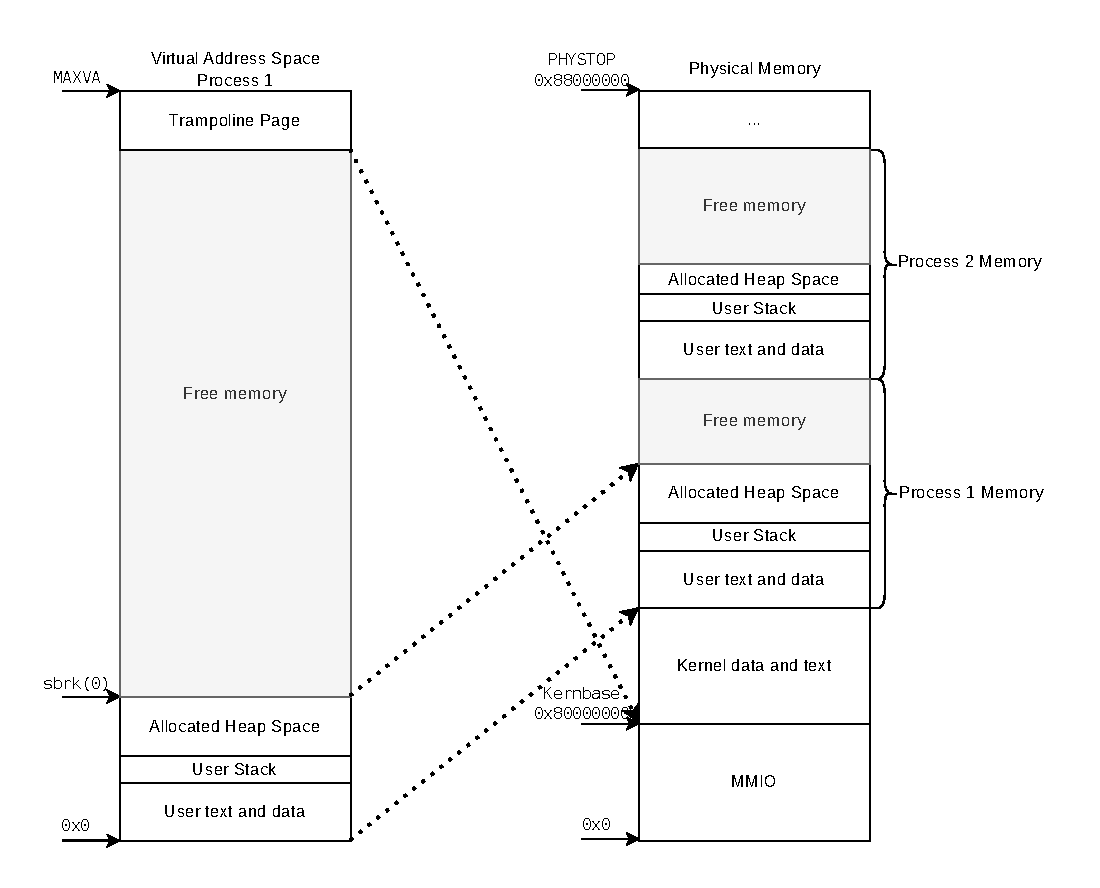
\includegraphics[]{figures/simple_mapping.pdf}

    \caption[Simple Mapping Scheme]{Simple Mapping Scheme}
    \label{fig:theory:simplemapping}
\end{figure*}
\chapter{Related Work}

\label{chap:related}

% \section{Liedtke: Guarded Page Tables}
% \todo{Should this be in the fundamentals chapter? Inverted Page tables are used relatively much}
% \section{Inverted Page Tables}

% \section{Other software-based TLB miss handlers / Page table walkers?}

\begin{itemize}
    %
    \item Software Managed Address Translation
    \item
\end{itemize}

This is just a little Test at citing and how my citation will
look at the end \cite{jacobSoftwaremanagedAddressTranslation1997}


Another citation \cite{BuchananRSS08}
\chapter{Theory}

\label{chap:theory}

\todo{a general motivation chapter about virtual memory should be in the fundamentals chapter}
\todo{Maybe motivation for VM on specific platforms like embedded platforms}
\section{Problem Statement}
%Reiteration of Problem Statement in introduction
\subsection{Der Trade-off von Hardware supported Virual Memory} % This is motivation
\section{Idea}
\section{L4/MIPS als Vorlage für Software TLB Management in RISCV (Qemu)}
\subsection{TLB Miss Exception}
\subsection{TLB Loading instructions}
\paragraph{tlbwi}
\paragraph{tlbwr}
\section{Motivation}
\subsection{Trade-offs of traditional Virtual Memory Approaches}





\chapter{Implementation}

\label{chap:impl}

\section{Platform}
\subsection{Platform Considerations}
% Which aspects are important for chosing the platform for this project?
% Why have I not chosen L4, Mips, etc? They already have some preconditions that are pretty good for my work (software handler, tlb instructions)
\subsection{xv6}
\subsection{RISC-V}
\subsection{Qemu}
\paragraph{softmmu Target}

\section{Modifying Qemu Source}
\subsection{TLB Miss Exception}
\subsection{CSR Modifications}
\subsubsection{TLB Modification via CSR}
\subsubsection{Switching between HW and SW TLB miss handling}

\section{xv6 TLB Miss Handler implementation Idea}
\subsection{code outline}
\subsection{Simplest case}
\subsection{Extrapolation target, most complex case}
\subsection{features to be implemented}
\subsection{realisation - how far have I come}

\section{Implementation description}
\subsection{Problems}
\subsection{idiosyncracies}
\subsection{limitations}
\chapter{Evaluation}

\label{chap:eval}

\section{performance?}
\subsection{Problems with measuring performance of an emulated system}
\chapter{Conclusion}

\label{chap:conclusion}


%----------------------------------------------------------------------------------------
%	THESIS CONTENT - APPENDICES
%----------------------------------------------------------------------------------------

% By using input instead of include for the chapters we are able to move the following line here
% Therefore the addition before the last chapter is not necessary anymore.

% Call the following chapters "Appendix" inside the table of contents
\addtocontents{toc}{\string\def\string\chaptername{Appendix}}

\appendix % Cue to tell LaTeX that the following "chapters" are Appendices

% Ensure proper section numbering in appendix, e.g., A.1, A.2, B.1, …
\renewcommand{\thesection}{\thechapter.\arabic{section}}
\renewcommand{\thesubsection}{\thesection.\arabic{subsection}}
\renewcommand{\thesubsubsection}{\thesubsection.\arabic{subsubsection}}

%%% CHANGES NEEDED HERE
%
% Include the appendices of the thesis as separate files from the Appendices folder
% Uncomment the lines as you write the Appendices

% Appendix A

\chapter{Unused paragraph dump}
\label{appendixa}


% Calling a function instead of doing a page table walk
The design presented here is based on the idea that virtual memory can be realized with a
mapping functions instead of the costly page table walks.\\
It may thus get rid of any state the memory system needs to keep book of mappings. The design
function that is to realize the mapping will only be based on its inputs. These inputs
should be found in the registers of the processor to avoid memory accesses as much as possible.

% How can software modify TLBs?
Running a function to generate mappings needs a computer with software-managed Virtual Memory.
MIPS provides some inspiration on how this can be done:\\
TLB misses throw a exception, the exception will be serviced by a kernel routine and the routine
uses specific instructions for writing to the TLB, thus resolving the TLB miss.


% Platform choice
The design will not be based on the MIPS platform, even though it already provides the hardware
features required to implement it.\\
Another requirement to the platform is simplicity and the availability of an easily comprehensible
and modifyable system running on top of it.\\
The xv6 is exactly such a system and there is a RISC-V implementation available.

% Why run on an emulator?
No real hardware is used to run the system, because the hardware needs to be extended to provide
the functionality of TLB miss exception throwing and TLB writing in order for the \emph{SoftTLB}
design to work.\\
The operating system will be run on the QEMU RISC-V emulator, which will be extended to satisfy
the extra functionality.


% About page table lookups
Figure \ref{fig:theory:mapping_fx} depicts the usual lookup approach of hierarchical page tables.
When the TLB misses, the MMU will perform a page table walk through the page table to retrieve the mapping
for the given virtual address.\\

% Inflexibility of HW VM
The specification of the MMU binds the software to a specific interface and page table structure. This restricts
the flexibilty of the software.

% MIPS SW Managed tlbs
To provide more flexibility, systems like MIPS allow for TLBs to be managed in software \cite{heiserAnatomyHighPerformanceMicrokernel}.
This still binds the operating system to adhere to the TLB structure, but leaves freedom on how the actual
entry is determined.\\

% Liedtke GPT
Virtual memory systems like Jochen Liedtkes Guarded Page Tables \cite{liedtkeGPT} use a table like structure
in combination with the flexible access to TLBs.\\

% Flexible tlb access enables alternative approaches
This flexibility also enables the implementation of alternative approaches that are not based on page tables,
but rather on mapping functions.\\

% Mapping function architecture
Figure \ref{fig:theory:mapping_fx} shows what the architecture of a system using a mapping function for
filling the TLB may look like.

% About mapping functions
In this paper, we want to take a closer look at such mapping functions and if a virtual memory system
can be realized without the usual bookkeeping cost of page tables.\\
Good candidates for such functions are non-cryptographic hash functions\todo{elaboration on hash functions}
to create a virtual to physical mapping.




%
With these changes, we implemented a system where TLB entries are populated using hash functions during TLB miss exceptions. This allows the virtual memory system to dynamically compute or retrieve the corresponding physical address without relying on multi-level page table walks, thus demonstrating a proof of concept for this alternative virtual memory approach.


%\chapter{More stuff} \todo{change chapoter name}
\label{appendixb}

%% Appendix C
 
\chapter{About the Template}
\label{appendixc}
\label{appendix-more-details-on-template}

This appendix provides additional information about less-often needed features of the template. Moreover, it contains a brief overview of the template's history. 

\section{Further Template Features}\label{ThesisFeatures}

This section explains customization options and technical details. For a thesis at the PSI Chair, you should stick with the defaults.

\subsection{Printing Format}

This thesis template is designed for double-sided printing (i.\,e., content on the front and back of pages) as most theses are printed and bound this way.\sidenote{At the PSI Chair, we highly encourage you to use double-sided printing.}
Switching to one-sided printing is as simple as uncommenting the \option{oneside} option of the \code{documentclass} command at the top of the \file{main.tex} file. You may then wish to adjust the margins to suit specifications from your institution.

The headers for the pages contain the page number on the outer side (so it is easy to flick through to the page you want) and the chapter name on the inner side.

The font size is set to 11 points by default with single line spacing; again, you can tune the text size and spacing using the options at the top of \file{main.tex}. The spacing can be influenced by replacing the \option{singlespacing} with \option{onehalfspacing} or \option{doublespacing}.

\subsection{Using US Letter Paper}

The paper size used in the template is A4, which is the standard size in Europe. If you are using this thesis template elsewhere, for instance, in the United States, then you may have to change the A4 paper size to the US Letter size.

Due to the differences in the paper size, the resulting margins may differ from what you like or require. You may need to adapt the page geometry settings in \file{setup.tex} in this case.

\subsection{References}

The template uses \code{biblatex} to format the bibliography and references such as this one \cite{murdoch_steven_j._chip_2010}. The template uses a citation style that creates in-text citations with the author(s) initials and the year of the publication. Multiple references are separated by semicolons (e.\,g., \cite{solat_security_2017, bond_chip_2014}). To see how you use references, look at the source files of this guide. If you choose a suitable BibTeX reference manager, you can copy and paste or drag and drop references into the document.

The bibliography is typeset with references listed in alphabetical order by the first author's last name. To see how LaTeX typesets the bibliography, look at the end of this document (or just click on the reference links in in-text citations).

\paragraph{BibTeX Backend}

As the ``old'' \code{bibtex} backend does not correctly handle Unicode character encoding (i.\,e., ``international'' characters), we use the more modern \code{biber} BibTeX engine in this template.

Here, we cite a lot of references so that the list of references gets populated \cite{murdoch_steven_j._chip_2010,anderson_ross_emv:_2014,kou_weidong_secure_2003,solat_security_2017,bond_chip_2014,ortiz_s._is_2006,haselsteiner_security_2006,galloway_visa_2019,zhou_nshield_2014,lalehTaxonomyFraudsFraud2009,ferradiWhenOrganizedCrime2016,Yang10,Kopsell06,VilaGM03,Herrmann12-ipv6prefix,Herrmann14-diss,HBF:2013,Herrmann11-NordSec,AcarEEJND14,Herrmann09,WangG13,Raymond00,Hintz02,Herrmann14-encdns,Goodson12-privacy,WendolskyHF07,chaum81,BertholdFK00,Dingledine04,rfc5246,LoesingMD10,FuchsHF13}.



\section{Contributors and History}

This guide has been written by Dominik Herrmann. The LaTeX template has been created by Dominik Herrmann with support by Fabian Lamprecht. Dominik and Fabian are affiliated with the Privacy and Security in Information Systems Group at University of Bamberg (\url{https://www.uni-bamberg.de/psi/}).


The PSI Template has its own \emph{document class}, \file{PSIThesis.cls}. It has been derived from \file{MastersDoctoralThesis.cls} (\url{https://www.latextemplates.com/template/masters-doctoral-thesis}).

The MastersDoctoralThesis LaTeX thesis template is based initially on a LaTeX style file created by Steve R.\ Gunn from the University of Southampton (UK), department of Electronics and Computer Science. You can find his original thesis style file at his site at
\url{http://www.ecs.soton.ac.uk/~srg/softwaretools/document/templates/} (link not available as of 2019).

Steve's \file{ecsthesis.cls} was then taken by Sunil Patel, who modified it by creating a skeleton framework and folder structure for a thesis. The resulting template is available on Sunil's site at
\url{http://www.sunilpatel.co.uk/thesis-template}.

Sunil's template was made available through \url{http://www.LaTeXTemplates.com} where it was modified many times based on user requests and questions. Version 2.0 and onwards of this template represents a significant modification to Sunil's template and is, in fact, hardly recognizable. The work to make version 2.0 possible was carried out by \href{mailto:vel@latextemplates.com}{Vel} and Johannes Böttcher.


\section{License}
\label{sec:license}

We have chosen a license that  allows you to use the template for your thesis and make changes as needed. You are \emph{not} required to publish your thesis or its source code under the same license. If you fork the template or the guide, however, you have to comply with the following licensing restrictions.

This guide and the template are made available under the Creative Commons license 
CC BY-SA 4.0 (\url{http://creativecommons.org/licenses/by-sa/4.0/}) with two exceptions:

\begin{enumerate}
\item Some excerpts, figures, and tables in \Cref{Chapter2} and \Cref{appendixb} have been taken from the
literature. The respective elements are explicitly marked with a citation and a note
regarding the permission to re-use. They are not
covered by the CC license. Permission to re-use and distribute
these figures, tables, and excerpts must be obtained from the
respective copyright holders.

\item Parts of \Cref{Chapter1} and \Cref{appendix-more-details-on-template} contain content from the
MastersDoctoralThesis template mentioned above, which is licensed under 
CC BY-SA 3.0 (\url{http://creativecommons.org/licenses/by-nc-sa/3.0/}). 
The original content has been written by
Sunil Patel (\href{http://www.sunilpatel.co.uk}{www.sunilpatel.co.uk}) and
Vel (\href{http://www.LaTeXTemplates.com}{LaTeXTemplates.com}).
\end{enumerate}

As this guide contains copyrighted material from third parties, you cannot host your own copy of this guide online. Please use the URLs printed on the title page to link to this document.

The files \texttt{PSIThesis.cls}, \texttt{setup.tex}, and \texttt{titlepage.tex} are made available under
the LPPL v1.3c (\url{http://www.latex-project.org/lppl}).

The fonts that are included in this template in the \texttt{fonts} directory are licensed under the Apache License 2.0 (\emph{Roboto} sans-serif font) and the SIL OFL Version 1.1 (\emph{Iosevka} monospace font).




%----------------------------------------------------------------------------------------
%	BIBLIOGRAPHY
%----------------------------------------------------------------------------------------

% Bibliography has no wide margins:
\newgeometry{
	inner=2cm, % Inner margin
	outer=2cm, % Outer margin
	marginparwidth=0cm,
	marginparsep=0mm,
	bindingoffset=.5cm, % Binding offset
	top=1.5cm, % Top margin
	bottom=2.5cm, % Bottom margin,
	includehead,
	includefoot
	% showframe, % Uncomment to show how the type block is set on the page
}

\addchap{References}

% enables two-column layout for bibliography
\setlength\columnsep{2em}
\begin{multicols}{2}
	\begin{refcontext}[sorting=nyt] % sort bibliography by last name, year, title
		\renewcommand*{\bibfont}{\small\RaggedRight}
		\linespread{1.0}\selectfont % increase linespread if desired (not recommended)
		\printbibliography[heading=none]
	\end{refcontext}
\end{multicols}

%----------------------------------------------------------------------------------------

%----------------------------------------------------------------------------------------
%	DECLARATION PAGE
%----------------------------------------------------------------------------------------

\begin{declaration}
	\addchaptertocentry{\authorshipname} % Add the declaration to the table of contents

	% TODO Change the declaration according as needed. *

	%\selectlanguage{ngerman}
	Ich erkläre hiermit gemä\ss\ \S~9 Abs.\,12 APO, dass ich die vorstehende {\thesistype}arbeit selbständig verfasst und keine anderen als die angegebenen Quellen und Hilfsmittel benutzt habe. Des Weiteren erkläre ich, dass die digitale Fassung der gedruckten Ausfertigung der {\thesistype}arbeit ausnahmslos in Inhalt und Wortlaut entspricht und zur Kenntnis genommen wurde, dass diese digitale Fassung einer durch Software unterstützten, anonymisierten Prüfung auf Plagiate unterzogen werden kann.

	\bigskip
	\bigskip

	\begin{tabular}{@{}l@{}}
		Bamberg, den \rule[-0.8em]{10em}{0.5pt} \\[2ex]
		~
	\end{tabular}
	\hspace{\fill}%
	\begin{tabular}{@{}c@{}}
		\rule[-0.8em]{20em}{0.5pt} \\[2ex]
		\authorname
	\end{tabular}\hspace{\fill}




\end{declaration}

\end{document}
